\section{Dynamic Adaptive Streaming over HTTP}
\begin{figure}[!t]
	\centering
	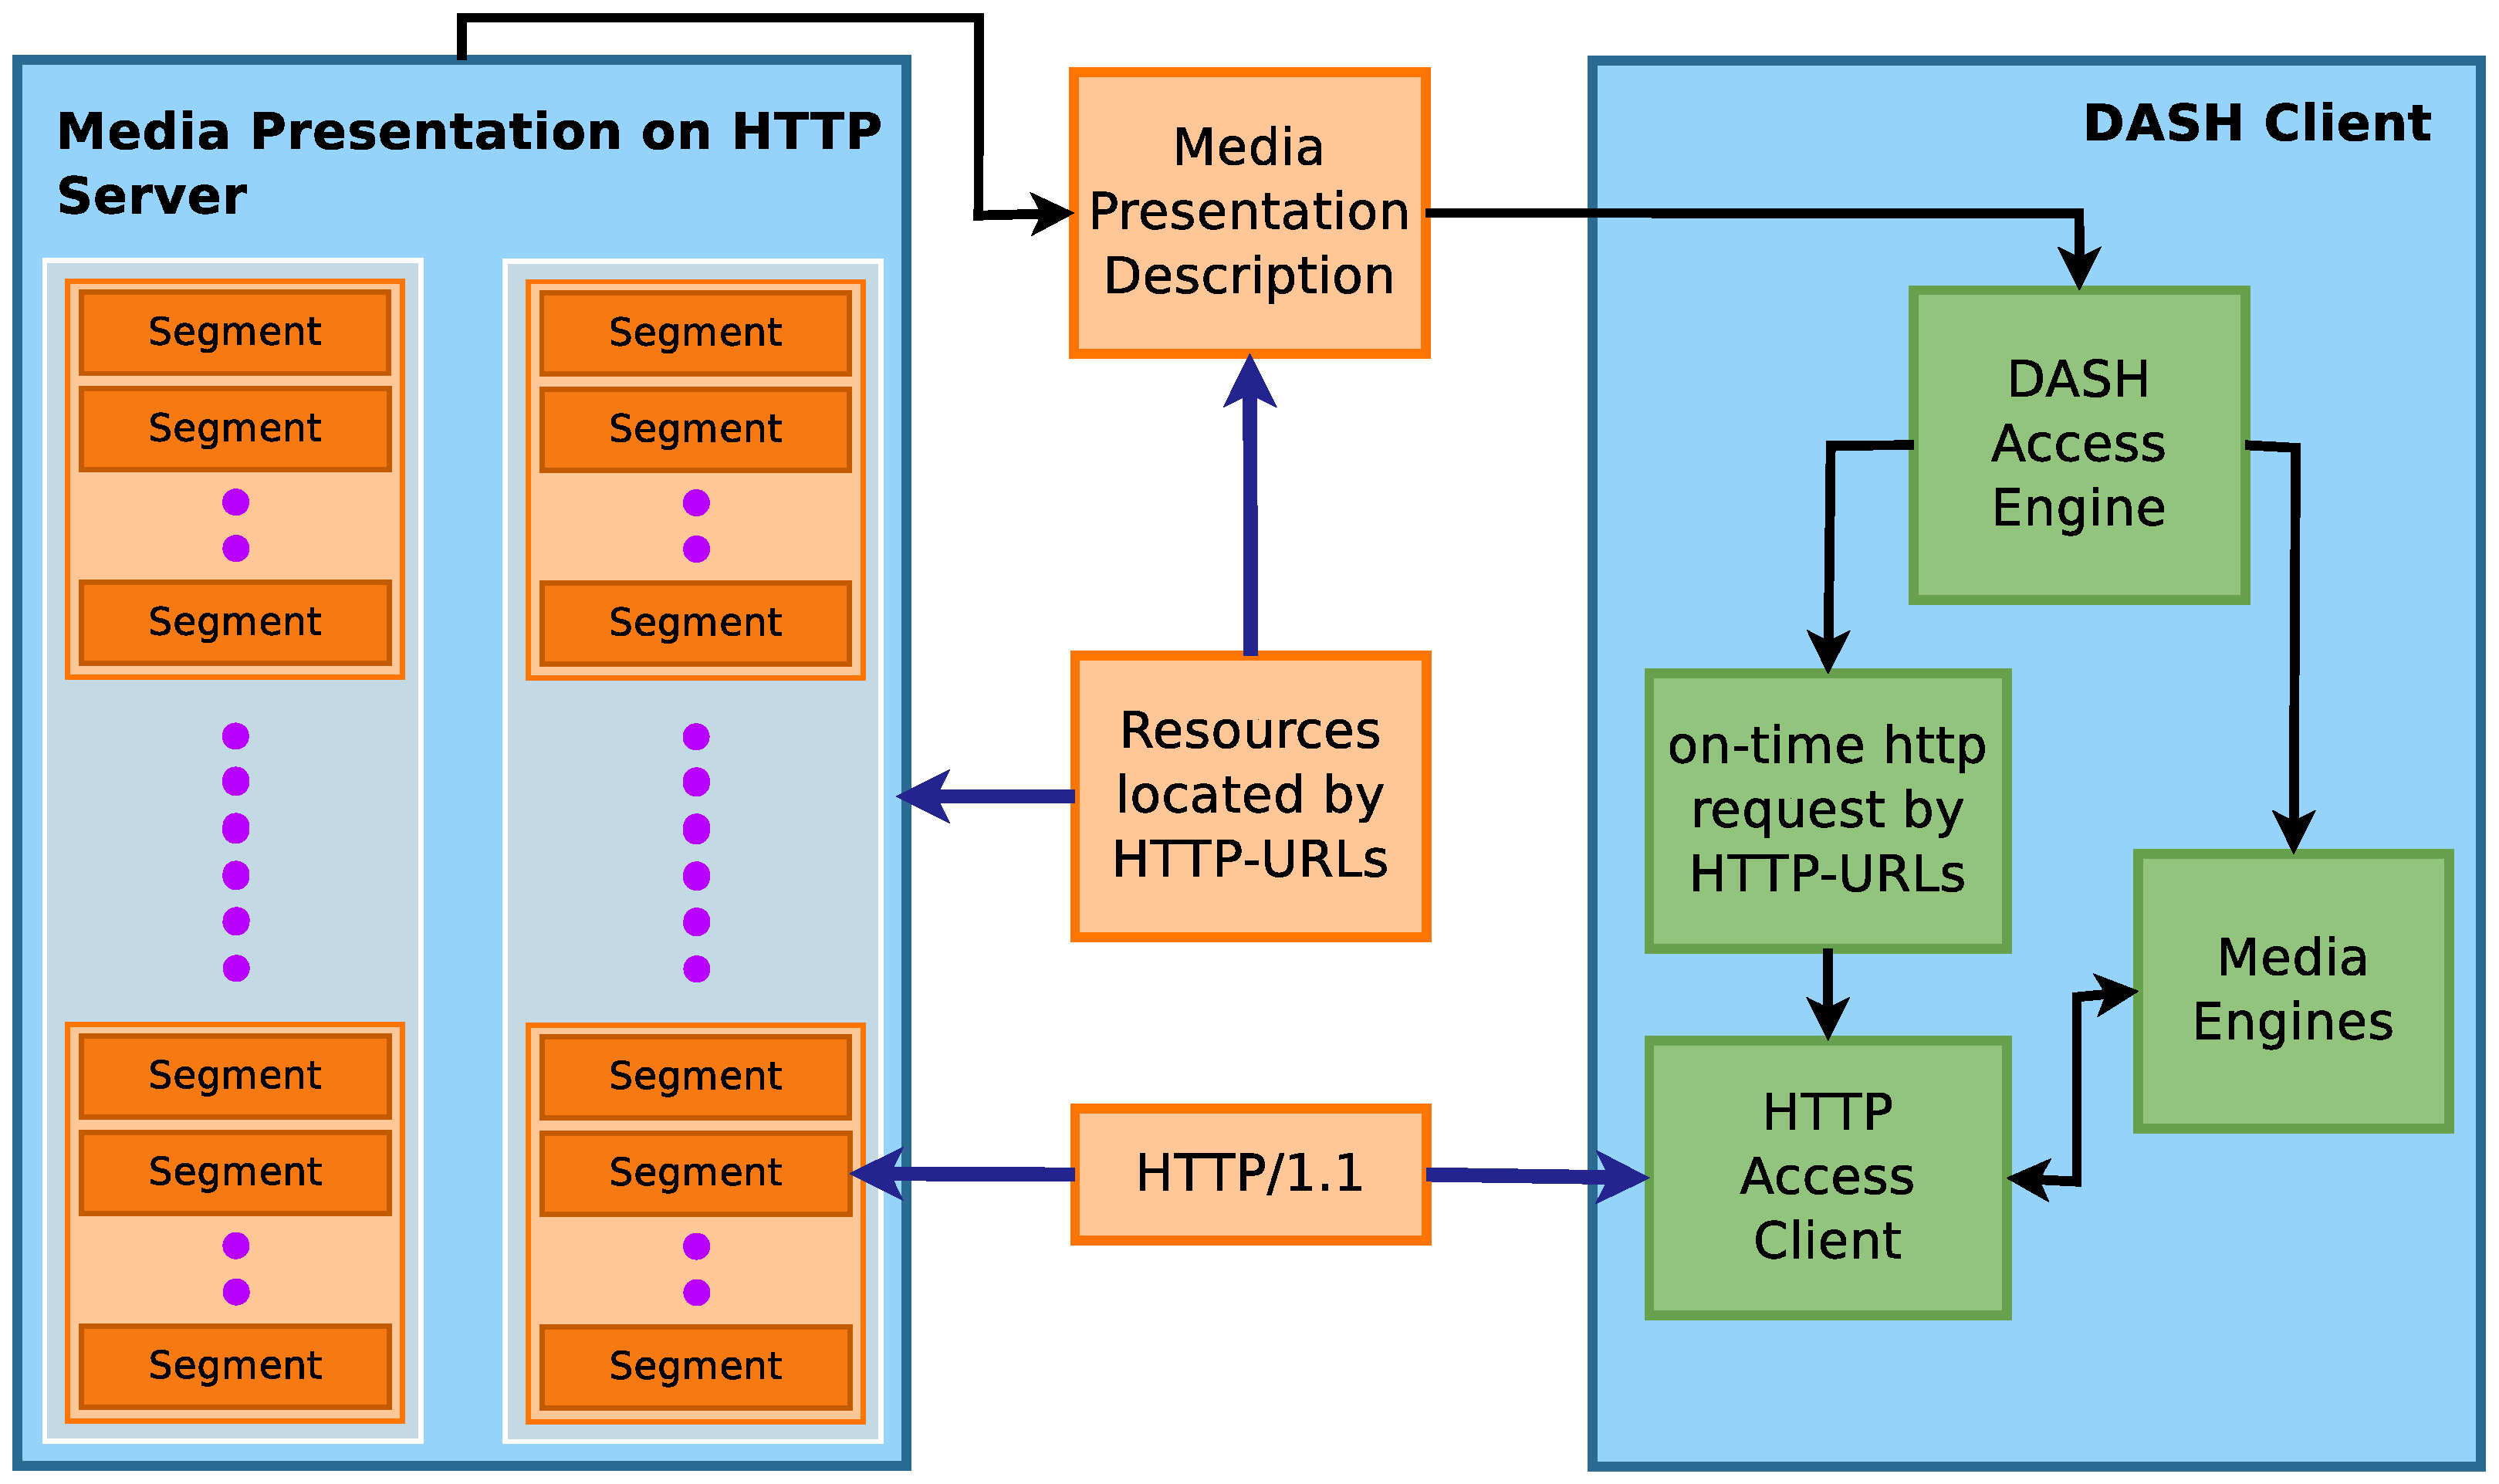
\includegraphics[scale=0.15]{img/dash-arch}
	\caption{\small{DASH Architecture -- On the left side, the server-side media storage is shown, where content is divided into small segments of alternative bit-rates. On the right side, the DASH client architecture is shown; the {\it DASH Access Engine} monitors network bandwidth at the client and accordingly decides which segment to request from the server. (Image Source: https://www.w3.org/2011/09/webtv/slides/W3C-Workshop.pdf)}}
	\label{fig:dash}
\end{figure}
In 2009, Apple developed the HTTP Live Streaming to replace the existing RTSP based streaming for its QuickTime live streaming server\footnote{\url{https://appleinsider.com/articles/09/07/08/apple_launches_http_live_streaming_standard_in_iphone_3_0.html} (accessed: \today)}. Dynamic Adaptive Streaming over HTTP (DASH), sometimes calls as MPEG-DASH, is a technology developed under MPEG to stream video over HTTP. MPEG started working for DASH in 2010 and standardized in 2011\cite{ISO/IEC23009-1:2019}. After the release of {\tt dash.js} by DASH Industry Forum (DASH-IF), almost all the streaming services, including YouTube, NetFlix, Samsung, adopted the DASH in their services.

Video streaming using DASH is a two-step procedure: a) preprocessing video files to distribute and b) the streaming. In the preprocessing (we also call it DASHifying), the streaming provider needs to create the video's required files. It first split the audio and video stream and encode them into multiple bitrate variations. At this phase, the encoder needs to ensure that it aligns the I-frames \footnote{I-frame: a special type of frame that contains a complete picture and no-other frame required to render it. More details: \url{https://en.wikipedia.org/wiki/Video_compression_picture_types}} across different bitrate versions and place all the metadata at the beginning of the file. After encoding, three different types of files are created from the streams. These files are, i) media index files, ii) media data files, and iii) a media presentation description file.

{\bf Media index files:} In general, when any media data stored in a file, the file contain two pieces of information, a) the initialization part and b) the encoded media data. The initialization part contains information to decode the encoded data, which is a kind of index for the original media data. The DASH mandate that this initialization data should store in a separate file. So, while encoding video into different bitrate variation, the metadata part needs to be kept at the output file's beginning. The index files are usually smaller than any of the Media data, so it does not pose any overhead to the system.

{\bf Media data files:} The media data file contains the encoded media. According to DASH, media data are segmented in multiple chunks with equal playback time. All the segments should have an I-frame  at the beginning of the chunk.

{\bf Media presentation description:} It is a {\tt XML} file that contains the metadata required to stream the video. It lists the different audio and video quality available for stream and the URLs for the media index and media data. It also contains the codec, bitrate, and playback duration of individual chunks for each quality.

The preprocessing phase ends with placing all these different files in an HTTP(S) file server. DASH does not require anything else on the server-side to stream a video. It is valid for VoD as well as Live streaming. However, in live streaming, the segments need to be created on the fly and place in the server before any client requests it.

The second phase of the DASH based streaming is streaming the video. DASH requires a smart player that can understand the DASH and play the video. Whenever a player wants to play the DASH based video streaming, it first has to download the MPD file and read it to get other information regarding the stream. The player then has to decide which quality it wants to play based on the ABR algorithm running inside the player and get the preferred quality's chunk accordingly. DASH offloads the entire decision to the player so that any existing content delivery network can stream video content. There are instances where media index files and media data are not chunked instead kept in a fixed file. While this saved lot of disk space, the server have to support the HTTP range-request\footnote{\url{https://developer.mozilla.org/en-US/docs/Web/HTTP/Range_requests}}, and the player can get the desired chunk using the {\tt range} header.

DASH also allows streaming providers to support various client platforms and encode video in various codec and put all the information in the MPD file. Although the MPD file can get very big, the player can choose a platform supported codec and play it without any hassle.


\subsection{Adaptive Bitrate Algorithm}
The adaptive bitrate algorithm is the heart of the DASH based streaming system as it decides the quality of every segment on the fly. By default, the ABR algorithm runs just before fetching the next chunk. As the ABR algorithm is part of the player, it has access to all the playback related parameters, and it can use any of those parameters to decide quality for the next chunk. The primary goal of any ABR algorithm is to maximize Quality of Experience (QoE) so that users can enjoy the streaming in the best possible.

\subsubsection{Quality of Experience}
Quality of Experience is a crucial parameter in any field which involves end-users. In the case of video streaming, QoE is a metric to measure whether the user has enjoyed the video or not. QoE is mostly a user perspective, and it depends on several factors such as startup delay, quality fluctuations, overall quality, rebuffering, audio/video device, and video content. Although all these parameters are essential, it isn't easy to measure user-dependent parameter and video content. Several researchers tried to find the best measurable metric to calculate QoE, which can be acceptable. Mok \etal \cite{5990550} tried to estimate QoE from the network QoS. They suggested that user QoS (or QoS of HTTP) is the QoE. Research paper-like \cite{} tried to use Peak Noise to Signal Ratio (PSNR) and Structural Similarity Index Measurement (SSIM) as a parameter for QoE. Spiteri \etal\ considered only the rebuffering and average quality as QoE in their ABR algorithm BOLA\cite{7524428}. Yin \etal\cite{10.1145/2785956.2787486} proposes an equation (Eqn.~\ref{eqn:QoE}) to calculate QoE using four parameters:
\begin{itemize}
	\item {\bf Startup delay:} Delay before playback can be started. In the case of ABR based solution, startup delay depends on the efficient initial quality selection. Most of the ABR algorithms ignore this parameter and set initial quality as the lowest video quality available.
	\item {\bf Quality:} The sharpness of the video determines the quality of the video or audio. The sharpness of a video is directly related to the bitrate of sharpness increases. It is expected that sharp media have better media details in both audio and video, thus providing a better experience in enjoying the stream. Any ABR tries to maintain bitrate as high as possible so that the quality of the experience improves.
	\item {\bf Smoothness:} DASH allows the player to change video quality on the fly. Frequent quality change disrupts the smoothness of the video watching experience. So, ABR needs to minimize the quality change during playback.
	\item {\bf Rebuffering:} Rebuffering is the most irritating experience for any user. The entire DASH and DASH like system is developed just to minimize rebuffering. It outmost responsibility of any ABR to minimize the rebuffering by selecting appropriate quality based of the current network quality.
\end{itemize}
\begin{equation}
	\label{eqn:QoE}
	QoE = \sum_{i=1}^N q(R_i) - \lambda\sum_{i=1}^{N-1}\left|q(R_{i+1})-q(R_i) - \mu\sum_{i=1}^N \delta_i - \mu_s T_s\right|
\end{equation}
Eqn.~\ref{eqn:QoE} is use by most modern ABR algorithm which measure the QoE for video with $N$ segments where $R_i$ represent the bitrate of $i^{th}$ segment, $q(.)$ is utility function, $\delta_i$ is stall before $i^{th}$ and $\delta_0$ is always zero, $T_s$ is the startup delay. The $\lambda$, $\mu$ and $\mu_s$ are constant weights to define which parameters is more important.

To enhanced the online streaming experience researchers have developed various systems and ABR algorithms. We categorize ABR algorithms broadly in a) classical ABR algorithms and b) learning based ABR algorithms. In following section we discuss both of these ABR algorithms and systems specially designed for live streaming and smartphones.

%The ABR algorithms are part of the DASH based streaming client. Any player have to implement at least one ABR algorithm in there implementation to support the quality adaptation.
%
%The penetration of the smartphone and wide access to 4G-LTE cellular data is one of the many reason behind the popularity of DASH based streaming. All the major smartphone provide API to build DASH based streaming client using native player. Most of the smartphones also support HTML5 enable webview using which DASH based player can be developed at ease.
%
%\subsection{HTML5 and DASH}
%The world wide web consortium (W3C) specifies the experimental media source extension (MSE) which allow JavaScript to manuplate HTML5 video player directly. It also allows to push byte-stream of media data directly to the player decoder and change the player buffer as per requirement on-the-fly. The MSE provide a rich set of API which is being used to developed DASH based video streaming client as all the major browser support the MSE. With introduction of MSE, providing video streaming service become easier as no fancy player need to be installed in the user end and it become easier to update the player just by changing the {\tt JavaScript} player library.
